% ======================= Pre-Amble =========================
      
%Format
\documentclass[11pt, oneside]{article}   	% use "amsart" instead of "article" for AMSLaTeX format 
                     						%imports package {article} and specify option(s) [11pt, oneside]
\usepackage{geometry}                		% See geometry.pdf to learn the layout options. There are lots. 
    \geometry{letterpaper}                   		% ... or a4paper or a5paper or ... 
    %\geometry{landscape}                		% Activate for rotated page geometry

\usepackage[parfill]{parskip}    		        % Activate to begin paragraphs with an empty line rather than an indent

    %Colours
    \usepackage{graphicx, subcaption}
    \usepackage[usenames, dvipsnames]{color}     % font colour:    \textcolor{<colour>}{text}
          									%highlight text:  \colorbox{<color>}{text}
    \usepackage{soul}						%highlight text: \hl{}     %only  yellow								
    									%list of colours: https://www.sharelatex.com/learn/Using_colours_in_LaTeX
    									
    %Bullets
    \usepackage{enumerate}     %specify type of enumeration: \being{enumerate}[<type of enumeration>]
    
    %Footnote Spacing
    \setlength{\footnotesep}{0.4cm}                  %specify spacing b/w footnotes
    \setlength{\skip\footins}{0.6cm}                    % space b/w footnotes and textbody


%Mattematics
    %American Mathematics Society packages
    \usepackage{amsmath}	   %math
    \usepackage{amssymb}       %symbols
    \usepackage{amsthm}          %theorems

    %QED
    \newcommand*{\QEDA}{\hfill\ensuremath{\blacksquare}}         %make qed filled square:    \QEDA
    \newcommand*{\QEDB}{\hfill\ensuremath{\square}}               %make qed empty square: \QEDB 
    
    \renewcommand\qedsymbol{\ensuremath{\blacksquare}}		%Proof environment


%Figures
\usepackage{caption}
\captionsetup[figure]{labelfont=bf}    %make figure labels boldface
\captionsetup[table]{labelfont=bf}     %make table labels boldface

\usepackage[hidelinks]{hyperref}                % Allows for clickable references

    %Tables
    \usepackage[none]{hyphenat}                    % Stops breaking-up words in a table (i.e. no hyphens)                                                             
    
    \usepackage{array}   
    \newcolumntype{x}[1]{>{\centering\let\newline\\\arraybackslash\hspace{0pt}}p{#1}}       %center fixed column width: x{<len>}                      
    \newcolumntype{$}{>{\global\let\currentrowstyle\relax}}                                                   % let us apply things (e.g. bold/italicize) to entire row            
    \newcolumntype{^}{>{\currentrowstyle}}
    \newcommand{\rowstyle}[1]{\gdef\currentrowstyle{#1} #1\ignorespaces}
    
    %Images
    \graphicspath{ {images/} }                          %directory that your images are located in within your current directory
    
    %Diagrams
    \usepackage[latin1]{inputenc}
    \usepackage{tikz}
    \usepackage{tkz-berge}
    \usetikzlibrary{shapes,arrows}


%Bibliography
\usepackage[numbers,sort&compress]{natbib}   %for multiple references: sorts  (i.e. [1,2] NOT [2, 1] )
                                           				  %                                     compresses (i.e. [1-3] )
\usepackage[nottoc]{tocbibind}                            %add bibliography to table of contents


%Miscellaneous
\usepackage{dirtytalk}    %quotations: use \say  


%================== Header & Footer =========================
\usepackage{fancyhdr}
\usepackage{lastpage}      %ensures you can reference LastPage (i.e. Page 2 of 10)

\renewcommand{\headrulewidth}{0.4pt}		%Decorative Header line: thickness={0.4pt}
\renewcommand{\footrulewidth}{0.4pt}		%Decorative Footer line: thickness={0.4pt}

\setlength{\headheight}{13.6pt} 		%space b/w top of page & header
\setlength{\headsep}{0.3in}		%space b/w page header and body

%Make Header & Footer    
\pagestyle{fancy}
    \lhead{Stephanie Knill} 		% controls the left corner of the header
    \chead{} 					% controls the center of the header
    \rhead{} 					% controls the right corner of the header
    \lfoot{} 					% controls the left corner of the footer
    \cfoot{Page~\thepage\ of \pageref{LastPage}} 				% controls the center of the footer
    												%Page~\thepage\  if just want Page x
    \rfoot{}			 		% controls the right corner of the footer

% =============================== Document ===================================
\begin{document}

% Title Page
\title{MATH 302 --- Assignment 6 \\
\line(1,0){360} \\              %(slope x, y){length of line}
}
\author{
Stephanie Knill \\
54882113 \\
Due: March 2, 2016}

\date{}                   % Activate:  display a given date (e.g. {August 4} ) or no date (empty {} )
                                    %No activate: display current date
\maketitle

%\thispagestyle{empty}                   %Remove header from this (first) page. Change empty -> plain to keep numbering
%								-> Doesn't matter in this case (b/c title page)
%\cleardoublepage


% ================= Questions ================

\section*{Question 1: Section 5.1 \#21}

In a class of 80 students, a professor calls on 1 student chosen at random for a citation in each class period. There are 32 class periods in a term.

\begin{enumerate}[(a)]
	\item Let the random variable $X$ be the number of times a student is called upon in a term. Then the exact probability that a given student is called upon $j$ times during the term is given by
	\begin{align*}
		P(X=j) & = Bin(n,p) \\
		& = Bin(32, 1/80) \\
		& = {n \choose j} p^j \cdot (1-p)^{n-j} \\
		& = {32 \choose j} (1/80)^j \cdot (79/80)^{32-j}
	\end{align*}
	
	\item Using the poisson approximation to model $X$, we have $\lambda = np = 32 \cdot 1/80 = 2/5$. Thus for $j$ times
	\begin{align*}
		P(X=j) \approx Pois(\lambda) & = Pois(2/5) \\
		& = e^{-\lambda} \cdot \frac{\lambda^j}{j!} \\
		& = e^{-\frac{2}{5}} \cdot \frac{(2/5)^j}{j!} \\
	\end{align*}
	Thus for the probability for a given student called upon more than twice
	\begin{align*}
		P(X> 2) & \approx 1 - P(X=0) - P(X=1) \\
		& \approx 1 - e^{-\frac{2}{5}} \cdot \frac{(2/5)^0}{0!} - e^{-2/5} \cdot \frac{(2/5)^1}{1!} \\
		& \approx 1 - e^{-\frac{2}{5}} (1- \frac{2}{5}) \\
		& \approx 1 - e^{-\frac{2}{5}} \cdot \frac{3}{5} \\
		& \approx 0.598
	\end{align*}
	
\end{enumerate}

\section*{Question 2: Section 5.1 \#23}

\hl{I have on ducking clue....}

\section*{Question 3: Section 5.1 \#26}

Let the random variable $X$ be the number of hits on a square. Let the total number of hits be $n=537$ and the probability of being hit $p=\frac{1}{576}$. Assuming the hits were purely random, we can use the Poisson approximation with $\lambda = np = 537 \cdot \frac{1}{576} = \frac{537}{576}$ to find the probability that a particular square would have exactly $k$ hits:
\begin{align*}
	P(X=k) & \approx Pois(\frac{537}{576}) \\
	& \approx e^{-\frac{537}{576}} \cdot \frac{\frac{537}{576}^k}{k!}
\end{align*}
Let us now compute the expected number of squares that would have 0, 1, 2, 3, 4, and 5 or more hits. The probability a square has 0 hits is
\begin{align*}
	P(X=0) & \approx e^{-\frac{537}{576}} \cdot \frac{\frac{537}{576}^0}{0!} \\
	& \approx  e^{-\frac{537}{576}} \\
	& \approx 0.39
\end{align*}
Multiplying this by the number of square $n$ gives us the expected number of squares with 0 hits
\begin{align*}
	\text{Expected \# Squares} & = P(X=0) \cdot n \\
	& \approx 211.39
\end{align*}
Thus the expected number of squares to be hit 0 times is approximately 211. 

Although midterm season is no longer upon us, I honestly just don't give a duck. The remaining calculations were done in Python (Figure \ref{lazy}). 
    \begin{figure}[h]                                         
    \begin{center}
        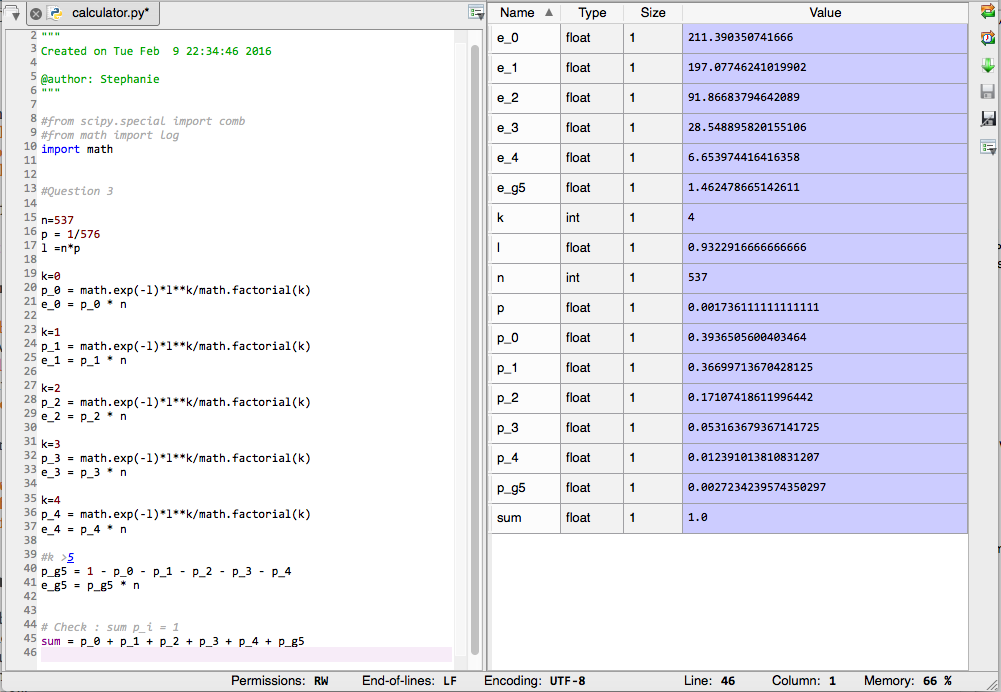
\includegraphics[width=.95\textwidth]{lazy.png}  
        \caption{Computation for the expected number of squares that would have 0, 1, 2, 3, 4, and 5 or more hits in Question 3.} 
        \label{lazy} 
    \end{center}
    \end{figure}
    
We have 211 squares with 0 hits, 197 with 1 hit, 92 with 0 hits, 29 with 3 hits, 7 with 4 hits, and 1 with 5 or more hits. Although only an approximation, they are still comparable to the observed results (229 squares with 0 hits, 211 with 1 hit, 93 with 0 hits, 35 with 3 hits, 7 with 4 hits, and 1 with 5 or more hits).

\section*{Question 4: Section 2.2 \#1}

Let us choose a \textit{random} (i.e. uniform/equiprobable density) real number $X$ from the interval [2,10].
\begin{enumerate}[(a)]
	\item The density function $f(x)$ can be computed as
	$$f(x) = \frac{1}{\text{length of interval}} = \frac{1}{10-2} = \frac{1}{8}$$
	and the probability of an event $E$ that is a subinterval $[a,b]$ of [2.10] as
	$$P(E) = \frac{\text{length of } E}{\text{length of interval}} = \frac{b-a}{8}$$
	
	\item For the probability that $X>5$, we have
	\begin{align*}
		P(X>5) & = 1 - P(X \leq 5) \\
		& = 1 - \frac{5-2}{8} \\
		& = \frac{5}{8}
	\end{align*}
	Similarly for $5 < X < 7$
	\begin{align*}
		P(5 < X < 7) & = 1 - P(X \leq 5) - P(X \geq 7) \\
		& = 1 - \frac{5-2}{8} - \frac{10-7}{8} \\
		& = \frac{1}{4}
	\end{align*}
	For $X^2-12X+35>0$, we can simplify this to
	\begin{align*}
		X^2-12X+35 = (X-7)(X-5) > 0
	\end{align*}
	Thus $X>7$ or $X<5$. Computing the probability
	\begin{align*}
		P(5 < X < 7) & = P(X > 7 \cup X <5) \\
		& = P(X > 7) + P(X<5) - P(X> 7 \cap X < 5) \\
		& = P(X > 7) + P(X<5) \\
		& = 1 - P(X \leq 7) + 1 - P(X \geq 5) \\
		& = 2 - \frac{7-2}{8} - \frac{10-5}{8} \\
		& = \frac{3}{4}
	\end{align*}
\end{enumerate}


\section*{Question 5: Section 2.2 \#2}

Let us choose a real number $X$ from the interval [2,10] with a density function of the form
$$f(x) = Cx,$$
where $C$ is a constant.
\begin{enumerate}[(a)]
	\item To compute $C$, we will use the fact that the 
	$$\int_a^b f(x)  \; \mathrm{d}x = 1$$	
	Here, $[a,b] = [2,10]$ so we have
	\begin{align*}
		\int_2^{10} Cx\;\mathrm{d}x & = 1 \\
		C \cdot \frac{x^2}{2} \Big|_{x=2}^{10} & = 1 \\
		C & = \frac{1}{48}
	\end{align*}
	
	
	\item The probability of an event $E$ that is a subinterval $[a,b]$ of [2.10] is given by
	\begin{align*}
		P(E) & = \int_a^b f(x) \; \mathrm{d}x \\
		& = \frac{1}{16} x^2 \; \Big|_{x=a}^b \\
		& = \frac{b^2-a^2}{96}
	\end{align*}
	
	\item For the probability that $X>5$, we have
	\begin{align*}
		P(X>5) & = 1 - P(X \leq 5) \\
		& = 1 - \frac{5^2-2^2}{96} \\
		& = \frac{25}{32}
	\end{align*}
		
	
	Similarly for $X < 7$
	\begin{align*}
		P(5 < X < 7) & = 1 - P(X \geq 7) \\
		& = 1 - \frac{10^2-7^2}{96} \\
		& = \frac{15}{32}
	\end{align*}
	For $X^2-12X+35>0$, we have
	\begin{align*}
		P(5 < X < 7) & = P(X > 7) + P(X<5) \\
		& = 1 - P(X \leq 7) + 1 - P(X \geq 5) \\
		& = 2 - \frac{7^2-2^2}{96} - \frac{10^2-5^2}{96} \\
		& = \frac{3}{4}
	\end{align*}
\end{enumerate}

\section*{Question 6}

Let there be players $A$ and $B$ whom initially start with $i=\$10$ and $j=\$5$ respectively, giving us a total of $M=i+j = \$15$. Rolling a 6-sided fair die, player $A$ is paid $\$1$ from player $B$ if it is a 1 or 2, otherwise player $A$ pays $\$1$ to player $B$. So we have the probability of success for player $A$ to be $p=2/6 = 1/3$. Let $P_i$ be the probability player $A$ wins if  he or she has initially $i\$$ and $l_i = P_i - P_{i-1}$. To find an equation for $P_i$, we first compute $l_i$ to be
\begin{align*}
	P_i & = p \cdot P_{i+1} + (1-p) \cdot P_{i-1} \\
	p \cdot P_{i} + (1-p) \cdot P_{i} & = p \cdot P_{i+1} + (1-p) \cdot P_{i-1} \\
	(1-p) \cdot [P_i - P_{i-1}] & = p \cdot [P_{i+1} - P_i] \\
	(1-p) \cdot l_i & = p \cdot l_{i+1} \\
	l_{i+1} & = \frac{1-p}{p} \cdot l_{i} \\
	l_i & = \frac{1-p}{p} \cdot l_{i-1} \\
	l_i & = \alpha \cdot l_{i-1}
\end{align*}
where $\alpha = \frac{1-p}{p}$. Since $P_i$ can also be defined as the summation of all intervals up to $l_i$, we have
\begin{align*}
	P_i & = l_1 + l_2 + \ldots + l_i \\
	& = l_1 + \alpha \cdot l_1 + \ldots + \alpha^{i-1} \cdot l_1 \\
	& = l_1 \cdot (1 + \alpha + \ldots + \alpha^{i-1}) \\
	& = l_1 \cdot \frac{\alpha^i - 1}{\alpha-1} \\
	& = l_1 \cdot \frac{1-\alpha^i}{1-\alpha}
\end{align*}
Since $\alpha$ is known, let us compute the last remaining unknown, $l_1$. Using our boundary condition $P_M =1$ gives us
\begin{align*}
	P_M & = l_1 \cdot  \frac{1-\alpha^M}{1-\alpha} \\
	1 & = l_1 \cdot  \frac{1-\alpha^M}{1-\alpha} \\
	l_1 & = \frac{1-\alpha}{1-\alpha^M}
\end{align*}
Substituting back into $P_i$ gives us the desired equation
\begin{align*}
	P_i & = \frac{1-\alpha}{1-\alpha^M} \cdot \frac{1-\alpha^i}{1-\alpha} \\
	& = \frac{1-\alpha^i}{1-\alpha^M}
\end{align*}
Here, we have $i=10$, $M=15$, and $\alpha = \frac{1-p}{p} = \frac{2/3}{1/3} = 2$. Plugging this in
\begin{align*}
	P_i = \frac{2^10-1}{2^15-1} \approx 0.0312
\end{align*}
gives us the probability that player $A$ wins all his or her adversary's money to be approximately 3\%.


\end{document} 